\documentclass{beamer}

\mode<presentation>
{
  \usetheme{Boadilla}
  \usecolortheme{whale}
  \usefonttheme{default}
  \setbeamertemplate{navigation symbols}{}
  \setbeamertemplate{caption}[numbered]
} 
\usepackage{braille}
\usepackage[english]{babel}
\usepackage[utf8x]{inputenc}

\title{Misspelling}
\author[Boifava, Bregoli, Brenna]{ \\ Giulia Boifava, 781250 \\ Alessandro Bregoli, 780711 \\ Pietro Brenna, 781840}

\date{6 Luglio 2017}

\begin{document}

\begin{frame}
  \titlepage
\end{frame}

\section{Introduzione}

\begin{frame}{Introduzione}


    Gli odierni strumenti tecnologici quali smartphone, tablet e computer sono dotati di una serie di programmi e software che controllano
    l’ortografia delle parole digitate, correggendo automaticamente il termine scorretto o proponendo, in fase di digitazione, una serie di
    dizioni che più somigliano alle potenziali parole a cui si può riferire la sequenza di lettere già battute a tastiera.\\
    Il progetto da noi scelto (Misspelling) ha riproposto questo genere di problema, pertanto abbiamo scelto di provare a implementare 
    anche noi un correttore automatico di parole.

\end{frame}

\begin{frame}{Assunzioni sul dataset}
Per semplicità grammaticale e lessicale abbiamo scelto la lingua inglese in quanto scarsa o priva di determinati simboli (accenti) e generi (maschile / 
femminile).
Inoltre abbiamo effettuato un’ulteriore scrematura non considerando simboli di punteggiatura e caratteri speciali quali “\#”, “-“, “@” e simili, ma 
considerando solamente le lettere.

La piccola modifica che abbiamo effettuato rispetto alla specifica, è il fatto di aver preso in considerazione come dataset un libro di narrativa in 
lingua inglese, invece che i Tweet del famoso Social Network.
\end{frame}

\begin{frame}{Dataset}
Il dataset che abbiamo scelto è composto da testi di romanzi quali:
\begin{itemize}
 \item Il signore degli Anelli
 \item Harry Potter
 \item Dune
\end{itemize}
La ragione di questa scelta è data dal fatto che il nostro modello prende in considerazione
la probabilità di una parola data la precedente.
\end{frame}



\begin{frame}{Scelte implementative}
Abbiamo sviluppato il progetto in linguaggio Python 3.6 e abbiamo aggiunto un ulteriore metodo di digitazione: oltre alla normale dicitura ed errori 
che possono incorrere digitando su una tastiera qwerty, abbiamo anche preso in considerazione i problemi che possono sorgere utilizzando una tastiera 
Braille.

L’interfaccia è stata sviluppata in HTML. Una volta digitata la parola appare un menù con una lista di 6 alternative, scelte dal programma in base 
all’adiacenza di eventuali lettere scritte per errore.
\end{frame}
\begin{frame}{Modello}
\begin{itemize}
 \item Per la tastiera qwerty abbiamo considerato adiacenti le lettere vicine. Per esempio, le lettere adiacenti alla “a” sono “q”, “w”, “s”, “z”.
 \item Per la tastiera Braille, invece, abbiamo considerato adiacenti le lettere che differiscono l’una dall’altra per la presenza o meno di un 
puntino. Per esempio, abbiamo considerato adiacenti alla “d” (\braille{d}) i caratteri “g” (\braille{g}), “n” (\braille{n}),  “c” (\braille{c}), “e” 
(\braille{e}).
\end{itemize}
\end{frame}

\begin{frame}{Metodo}
 Operiamo con un hidden markov model in cui:
 \begin{itemize}
  \item gli stati corrispondono alle parole intere
  \item l'osservazione corrisponde alle lettere digitate per formare la parola
  \item la transizione è data dalla probabilità di una parola data la precedente, calcolata sul dataset.
 \end{itemize}
 In più viene costruito a partire dal dataset un insieme di parole corrette ("dizionario").
\end{frame}

\begin{frame}{Modello di osservazione}
 Come calcolare la probabilità di uno stato (parola) data l'evidenza (lettere digitate)?
 
 Partiamo dall'intuizione di fondo della edit distance e creiamo una funzione di edit probability, che dà la probabilità di aver digitato una certa 
evidenza avendo inteso digitare una certa parola. Tale funzione si appoggia ad un modello di digitazione (tastiera o braille nel nostro caso).
 
 \end{frame}
 
 \begin{frame}{Edit Probability}
 	    \begin{table}
    \centering
    \begin{tabular}{l|l|l|l|l|l}
               & $\epsilon$ & c        & i        & a        & l \\ \hline
	$\epsilon$ & 1.0        & 0.05     & 0.0025   & 0.000125  & 6.25e-06    \\
    c          & 0.02       & 0.92     & 0.0184   & 0.000368  & 7.36e-06    \\
    i          & 0.0004     & 0.046    & 0.8464   & 0.016928  & 0.00033856  \\
    a          & 8e-06      & 0.0023   & 0.04232  & 0.778688  & 0.01557376  \\
    o          & 1.6e-07    & 0.000115 & 0.002116 & 0.0389344 & 0.00648906  \\

    \end{tabular}
    \caption{Calcolo della edit probability di "ciao" dato "cial"}
    \end{table}
 \end{frame}
 
 \begin{frame}{BK-Tree}
 	Tuttavia la edit probability risulta essere lenta e dunque è stata implementata la
 	struttura dati BK-Tree che risulta essere più efficiente nel selezionare parole
 	 sintatticamente vicine	a quella digitata. 
 	 \pause
 	 \begin{center}
 	 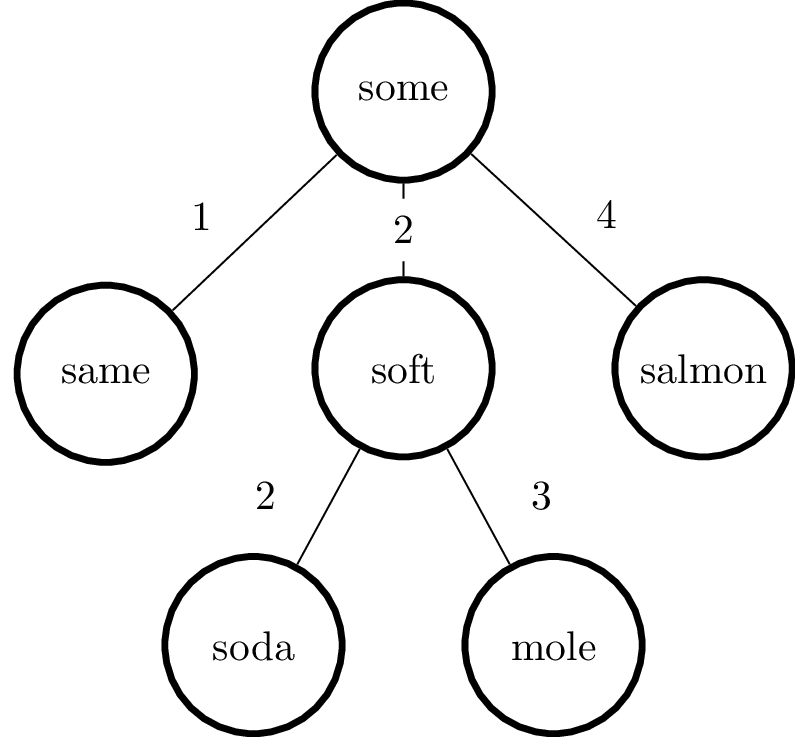
\includegraphics[width=0.5\textwidth]{bk-tree.png}
 	 \end{center}
\end{frame}

\begin{frame}{Correzione errori}
 Una volta costruito tale modello, l'algoritmo di Viterbi ci restituisce la sequenza più probabile di parole. È importante notare che tutte le parole 
restituite dall'algoritmo di Viterbi provengono dal dizionario.
\end{frame}

\begin{frame}{Risultati}
 Per validare il progetto abbiamo preso un testo e abbiamo alterato circa una lettera ogni 30 per avere mediamente una parola errata ogni 7-8. 
Misuriamo la percentuale di parole corrette prima e dopo aver applicato l'algoritmo di correzione.\\
\vspace{0.5cm}
 
 \centering
 \begin{tabular}{|c|c|c|}
 \hline
  \textbf{Testo} & \textbf{Perturbazione} & \textbf{Errore residuo}\\
 \hline
 	test1 & 16\% &  3\% \\
 \hline 
    test2 & 12\% & 5\%\\
 \hline
 \end{tabular}
\end{frame}

\begin{frame}{Conclusioni}
  I maggiori problemi dipendono dal fatto che l'HMM è del primo ordine dunque ogni parola dipende solo dalla propria distanza rispetto a quella 
digitata 
  e dalla parola precedente; inoltre non tiene in considerazione la semantica della frase. In generale il modello corregge con maggiore accuratezza 
frasi
  brevi.
\end{frame}
\begin{frame}{Possibili miglioramenti}
	Possibili sviluppi futuri potrebbero essere:
    \begin{itemize}
    	\item Utilizzo di un modello HMM di ordine superiori al primo
        \item Considerazione della logica della frase utilizzando NER
        \item Parallelizzazione di alcuni task in modo da rendere il modello più scalabile
    \end{itemize}
\end{frame}
\end{document}
